%%%%%%%%%%%%%%%%%%%%%%%%%%%%%%%%%%%%%%%%%%%%%%%%%%%%%%%%%%%
% --------------------------------------------------------
%     BIBLIOGRAPHY WITH BIBLATEX IN EXTERNAL EDITORS
% --------------------------------------------------------
% If the bibliography does not show up, try running the 
% 'tau.cls' and 'tau.bib' file with biber from the 
% MikTeX console or your preferred LaTeX distribution to 
% generate the auxiliar files and (re)run the main.tex.
% --------------------------------------------------------
%%%%%%%%%%%%%%%%%%%%%%%%%%%%%%%%%%%%%%%%%%%%%%%%%%%%%%%%%%%
% --------------------------------------------------------
%					  FOR SPANISH BABEL
% --------------------------------------------------------
% \usepackage[spanish,es-nodecimaldot,es-noindentfirst]{babel}
% --------------------------------------------------------
%%%%%%%%%%%%%%%%%%%%%%%%%%%%%%%%%%%%%%%%%%%%%%%%%%%%%%%%%%%

\documentclass[10pt,a4paper,twoside]{tau}
\usepackage[english]{babel}
\usepackage{tauenvs}
\usepackage{xcolor}
\usepackage{hyperref}
\hypersetup{
    colorlinks=true,
    linkcolor=brown,
    urlcolor=blue,
    citecolor=red,
}
\renewcommand{\vec}[1]{\mathbf{#1}}
\renewcommand{\d}{\text{d}}
%----------------------------------------------------------
% TITLE
%----------------------------------------------------------

\title{Image Classification Based On Three-Layer Neural Network}

%----------------------------------------------------------
% AUTHORS, AFFILIATIONS AND PROFESSOR
%----------------------------------------------------------

\author[]{Xiang Zheng, 21307110169}

%----------------------------------------------------------

\affil[]{School of Data Science, Fudan University}

%----------------------------------------------------------
% FOOTER INFORMATION
%----------------------------------------------------------

\institution{}
\ftitle{}
\date{}
\etal{}
\course{Computer Vision}

%----------------------------------------------------------
% ABSTRACT
%----------------------------------------------------------

\begin{abstract}
This project focuses on developing and training a neural network to accurately classify grayscale fashion items in the Fashion-MNIST dataset. The neural network architecture consists of three linear layers, with a thorough exploration of activation functions and loss functions to optimize performance. The report covers dataset acquisition, architectural decisions, training procedures, and evaluation metrics, underscoring the importance of meticulous design and optimization in neural network development for image classification tasks. The trained model achieves a training accuracy of $94.8\%$ and a testing accuracy of $89.6\%$.
\end{abstract}
\keywords{Fashion-MNIST, image classification, neural network}

%----------------------------------------------------------

\begin{document}
		
\maketitle
\thispagestyle{firststyle}
\tauabstract

%----------------------------------------------------------

\section{Introduction}

\taustart{I}n this project, our goal is to train a fully connected neural network to classify images from the Fashion-MNIST dataset. Curated by Zalando, this dataset contains grayscale images of various fashion items, along with corresponding category labels. With 60,000 training examples and 10,000 test examples, Fashion-MNIST serves as a standard benchmark for fashion image classification.

Our neural network consists of three linear layers, trained to learn meaningful representations and make accurate predictions. We explore various components like activation functions and training strategies to optimize performance. 

The remainder of this report is structured as follows: Section 2 provides the dataset acquisition and preprocessing method. Section 3 delves into the specifics of the neural network architecture, detailing the design choices for its components. Section 4 outlines the training process, including the selection of hyperparameters and evaluation metrics. In Section 5, we evaluate the trained model on the test dataset and present visualizations to assess its effectiveness. Finally, Section 6 discusses potential avenues for future improvement. 

\textbf{Note: You can find the project files in the \href{https://github.com/mango7789/Computer-Vision-HW1}{GitHub repo} and the model parameters in the \href{https://drive.google.com/file/d/1fHbpA-FtWAH-j2v-awv-D9p3sIjMfqLW/view?usp=drive_link}{Google Drive}. For instructions on how to train and test the neural network, please refer to the readme file. You can also directly preview the project files in \href{https://github1s.com/mango7789/Computer-Vision-HW1}{this website}.}



\section{Dataset}

Having already covered the dataset's characteristics earlier, we'll now delve straight into the downloading and preprocessing steps. Utilizing the Python library \texttt{urllib}, we'll fetch the data from its \href{https://github.com/zalandoresearch/fashion-mnist}{official repo} and organize it into a dictionary containing images and labels. Each numpy array representing a grayscale image will be reshaped into the format $(1, 28, 28)$ to maintain consistency with their original shapes.

\section{Model}

A standard linear layer neural network comprises three main components: the input layer, hidden layers, and output layer. The transition between the input (hidden) layer and hidden layers can be described as a \texttt{LinearActivation} layer, while the transition between the hidden layer and output layer involves a \texttt{Linear} layer along with a \texttt{loss} function. Other parameters like \texttt{reg} and \texttt{weight\_scale} also influence the performance of the model.

Before delving into the discussion of our model, it's essential to establish the key notations utilized throughout this report. Let $N$ represent the batch size, indicating the number of samples processed in each training or inference iteration. $D$ denotes the flattened dimension of the image, symbolizing the size of the image vector after flattening. $H_1, H_2, \cdots, H_n$ refer to the dimensions of the hidden layers within the neural network architecture. Finally, $C$ signifies the output dimension, representing the number of classes in the classification task.

\subsection{Linear Layer}

Consider the first linear layer as an illustration. The forward pass can be concisely expressed as:

\begin{equation}
    \vec{Y} = \vec{X}\vec{W} + \vec{b} \tag{3.1.1}
\end{equation}

Here, $\vec{Y} \in \mathbb{R}^{N \times H_1}$, $\vec{X} \in \mathbb{R}^{N \times D}$, $\vec{W} \in \mathbb{R}^{D \times H_1}$, and $\vec{b} \in \mathbb{R}^{H_1}$. It's worth noting that \texttt{numpy} broadcasts $\vec{b}$ to fit into the computation. Hence, we represent $\vec{b}$ as a vector to maintain alignment with my code implementation. Also, please note that we need to 'cache' the current values of $\vec{X}$ and $\vec{W}$ for the backward pass.

Regarding the backward pass, the input of the backward function is \texttt{dout} and \texttt{cache}, where \texttt{dout} represents the gradient at $\vec{Y}$ with shape $(N, H_1)$. Taking derivatives with respect to $\vec{X}$ and $\vec{W}$, we obtain:

\begin{equation}
    \d\vec{X} = \d\vec{Y} \cdot \vec{W}^{\top} \tag{3.1.2}
\end{equation}
\begin{equation}
    \d\vec{W} = \vec{X}^{\top} \cdot \d\vec{Y} \tag{3.1.3}
\end{equation}
For bias $\vec{b}$, the derivative involves summing \texttt{dout} over the first dimension. 


\subsection{Activation Functions}

When it comes to activation functions, they all perform an element-wise operation on the given matrix. There are several commonly used types of activation functions, including \texttt{ReLU}, \texttt{Tanh}, and \texttt{Sigmoid}. Let's introduce each of them individually.

\subsubsection{ReLU}

For the forward pass, ReLU is expressed as:
\begin{equation}
\vec{Y'} = \max(\vec{Y}, \vec{0}) \tag{3.2.1}
\end{equation}
For the backward pass, it's:
\begin{equation}
\d\vec{Y} = \max(\d\vec{Y'}, \vec{0}) \tag{3.2.2}
\end{equation}

\subsubsection{Tanh}

The mathematical expression of the hyperbolic tangent function, Tanh, is:
\begin{equation}
\tanh{x} = \frac{e^{2x} - 1}{e^{2x} + 1} \tag{3.2.3}
\end{equation}
Taking the derivative with respect to $x$, we get:
\begin{equation}
\frac{\partial \tanh{x}}{\partial x} = \frac{4}{(e^{2x}+1)^2} = 1 - \tanh^2{x} \tag{3.2.4}
\end{equation}

The forward and backward pass follows directly from the above equations:
\begin{equation}
\vec{Y'} = \tanh{\vec{Y}} \tag{3.2.5}
\end{equation}
\begin{equation}
\d\vec{Y} = \d\vec{Y'}\cdot(1 - \tanh^2\vec{Y}) \tag{3.2.6}
\end{equation}

\subsubsection{Sigmoid}

Let's denote the sigmoid function as:
\begin{equation}
\sigma(x) = \frac{1}{1 + e^{-x}} \tag{3.2.7}
\end{equation}
Taking the derivative with respect to $x$, we obtain:
\begin{equation}
\frac{\partial\sigma(x)}{\partial x} = \frac{e^{-x}}{(1 + e^{-x})^2} = \sigma(x)(1 - \sigma(x)) \tag{3.2.8}
\end{equation}
Then, the forward and backward pass of the sigmoid function are:
\begin{equation}
\vec{Y'} = \sigma(\vec{Y}) \tag{3.2.9}
\end{equation}
\begin{equation}
\d\vec{Y} = \d\vec{Y'}\cdot \sigma(\vec{Y}) (1 - \sigma(\vec{Y})) \tag{3.2.10}
\end{equation}

\subsection{Loss Function}

The loss function plays a crucial role in training a neural network as it quantifies the discrepancy between the predicted output and the actual target. Here, we'll implement the \texttt{cross\_entrophy}. Since this is a multi-class classification task, the CE is slightly different from the binary case.

For traditional binary cross entropy, the loss function is

\begin{equation}
    \text{loss}(\vec{y}, \vec{\hat{y}}) = -\frac{1}{N} \sum_{i=1}^{n}y_i
    \log(\hat{y}_i) + (1 - y_i) \log(1 - \hat{y}_i) \tag{3.3.1}
\end{equation}

where $y_i$ can only take the value of 0 or 1. However, this is not appropriate in multi-class classification.

To compute the loss function in the forward pass of the neural network, we'll first apply the softmax function to the raw output scores to obtain the predicted probabilities for each class. The softmax function is defined as:

\begin{equation}
\text{softmax}(\vec{x})_i = \frac{e^{x_i}}{\sum_{j=1}^{C} e^{x_j}} \tag{3.3.2}
\end{equation}

where $\vec{x}$ is the vector of raw output scores, and $C$ is the number of classes. This function ensures that the predicted probabilities are normalized and sum up to $1$ for each sample. Besides, the 'shifted x' method is used here to avoid overflow.

Once the softmax probabilities are computed, the cross-entropy loss can be calculated using the true labels and the predicted probabilities. The cross-entropy loss is defined as:

\begin{equation}
\text{CE} = -\frac{1}{N} \sum_{i=1}^{N} \sum_{s=1}^{C} t_{i,s} \log(f(s)_i) \tag{3.3.3}
\end{equation}

where $N$ is the number of samples, $C$ is the number of classes, $t_{i,s}$ is the true label for the $i$-th sample and $s$-th class (which is $1$ if the sample belongs to class $s$ and $0$ otherwise), and $f(s)_i$ is the predicted probability for the $i$-th sample belonging to the $s$-th class. Hence the loss can be further simplified as
\begin{equation}
    \text{CE} = -\frac{1}{N} \sum_{i=1}^{N} t_i \log(f(s)_i) \tag{3.3.4}
\end{equation}

In the backward pass, we'll need to compute the gradient of the loss function with respect to the raw output scores. This involves subtracting the true labels from the softmax probabilities, resulting in the gradient matrix. The gradient can be calculated as:

\begin{equation}
\frac{\partial \text{CE}}{\partial \mathbf{x}} = \frac{1}{N} (\text{softmax}(\mathbf{x}) - \mathbf{t}) \tag{3.3.5}
\end{equation}
and it's implemented in Python code as
\begin{center}
\begin{lstlisting}[language=Python,
        stringstyle=\color{green},
        numbers=none,
        keywordstyle=\color{purple},
        keywords={np, arange, sum, copy, exp}
    ]
# probs denotes the softmax result
probs = np.exp(log_probs)
loss = -np.sum(log_probs[np.arange(N), y])
loss /= N
dx = np.copy(probs)
dx[np.arange(x), y] -= 1
dx /= N
\end{lstlisting}   
\end{center}


\subsection{Other Parameters}

In addition to the model architecture, such as linear and activation layers, neural networks often involve hyperparameters such as \texttt{hidden\_dims}, \texttt{reg}, and \texttt{weight\_scale}. 

For \texttt{hidden\_dims} and \texttt{reg}, they determine the size of the hidden layers and serve as a regularization parameter that helps prevent overfitting by penalizing large weights in the model respectively. In the next section, we'll discuss how grid search is used to find the optimal values of them.

For \texttt{weight\_scale}, the initial scale of the weight matrix, a commonly recommended value is 0.01. This value provides a good starting point for weight initialization, ensuring that the network begins training with reasonable weights.



%%%         train          %%%
\section{Train}

Now that we've covered the details of the Fully Connected Neural Network (FCNN) model in the previous section, let's delve into the training procedures. We'll begin by introducing some update rules, followed by a sanity check of the \texttt{Solver} on a small dataset to ensure its functionality. Subsequently, we'll conduct training for 2000 iterations for each configuration to identify the best configuration. Finally, the model will undergo training based on the optimal parameters for a significantly larger number of iterations to achieve the best results.

By the way, unless otherwise specified, the parameters used in this section are set to their default values, as detailed in Table \ref{tab:parameters}.


\begin{table}[htbp]
    \centering
    \begin{tabular}{|c|c|c|}
        \hline
        \textbf{Parameter Name} & \textbf{Default Value} \\
        \hline
        hidden\_dims & [128, 64]  \\
        \hline
        activation & [relu, relu] \\
        \hline
        reg & $1e^{-3}$ \\
        \hline
        update\_rule & sgd \\
        \hline
        learning\_rate & $5e^{-3}$ \\
        \hline
        lr\_decay & 0.9 \\
        \hline
    \end{tabular}
    \caption{Default value of parameters (partial listing)}
    \label{tab:parameters}
\end{table}

\subsection{Update Rule}

For update rules, we have provide four commonly used methods: stochastic gradient descent (SGD), SGD with momentum, Adam, and RMSprop. The mathematical explanation and some intuitions will be given below, while the experiment results of comparison of these four update rules will be defer to section 4.3.

\subsubsection{SGD}

The vanilla stochastic gradient descent is
\begin{equation}
    \vec{w} = \vec{w} - \texttt{lr} \cdot\d \vec{w} \tag{4.1.1}
\end{equation}
where the default value of \texttt{lr}(learning rate) is $1e^{-3}$.

\subsubsection{SGD Momentum}

For stochastic gradient descent with momentum, the update rule is 
\begin{equation}
    \vec{v} = \texttt{momentum} \cdot\vec{v} - \texttt{lr} \cdot\d\vec{w} \tag{4.1.2}
\end{equation}
\begin{equation}
    \vec{w} = \vec{w} + \vec{v} \tag{4.1.3}
\end{equation}
where $\vec{v}$ denotes the velocity. The empirical default values for \texttt{lr} and \texttt{momentum} are $1e^{-3}$ and $0.9$, respectively.

The advantages of SGD with momentum includes:
Momentum is faster than stochastic gradient descent the training will be faster than SGD. Local minima can be an escape and reach global minima due to the momentum involved. They'll be validated in the following experiments.

\subsubsection{Adam \& RMSprop}
Adam and RMSprop can be viewed as applying first-order and second-order normalization on the weight vector $\vec{w}$ respectively. These update rules are more complex compared to the ones discussed above. For a detailed explanation, please refer to the code implementation in \texttt{optimization.py}.


\subsection{Sanity Check}

For the sanity check, we trained the model using the first 500 samples of the training dataset for 2000 iterations. We set the hidden dimensions as $[128, 64]$ and used the \texttt{ReLU} activation function. The training results are depicted in Figure \ref{fig:sanity-check}:

\begin{figure}[hbp]
    \centering
    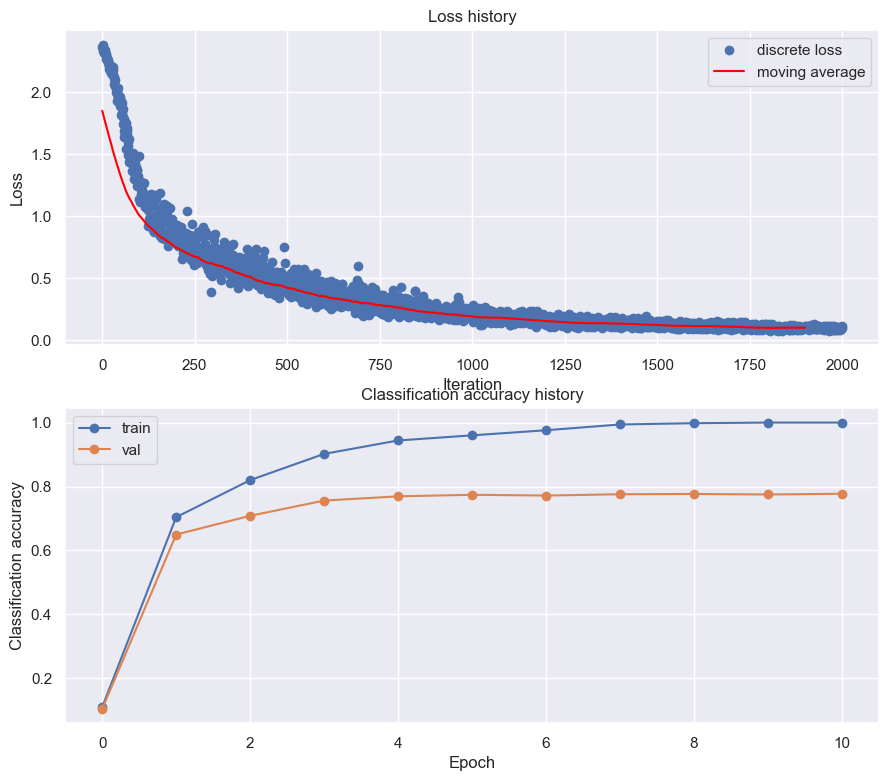
\includegraphics[scale=0.35]{images/sanity_check.png}
    \caption{Training on the Small Dataset}
    \label{fig:sanity-check}
\end{figure}

After 9 epochs of training (approximately 1800 iterations), the model achieved perfect accuracy on the training dataset, while the validation (testing) accuracy plateaued around 77.5\%. This indicates that our model is capable of overfitting the small subset of training data well, ensuring its availability for use. Now, let's proceed to fine-tune the model using the entire training dataset to find the best parameters.


\subsection{Search Best Configuration}

The process of searching the best configuration is divided into three subsections. First, the model will undergo training for 2000 iterations using 9 different combinations of activation functions while keeping other parameters constant to find the best combination, which can be seen as a greedy search. Subsequently, we will implement a grid search method to find the best hyperparameters \texttt{reg}, \texttt{learning\_rate}, and \texttt{hidden\_dims}. Finally, we will experiment with 4 different update rules mentioned in section 4.1.2 and compare their performance.


\subsubsection{Combinations Of Activation Functions}

As discussed in Section 3.2, we offer three commonly used activation functions: \texttt{ReLU}, \texttt{Tanh}, and \texttt{Sigmoid}. In a three-layer neural network, there are two layers for activation functions, leading to 9 different combinations.  The results of the experiments are presented in Figure \ref{fig:activation-loss} and Figure \ref{fig:activation-acc}.


\begin{figure}[htbp]
    \centering
    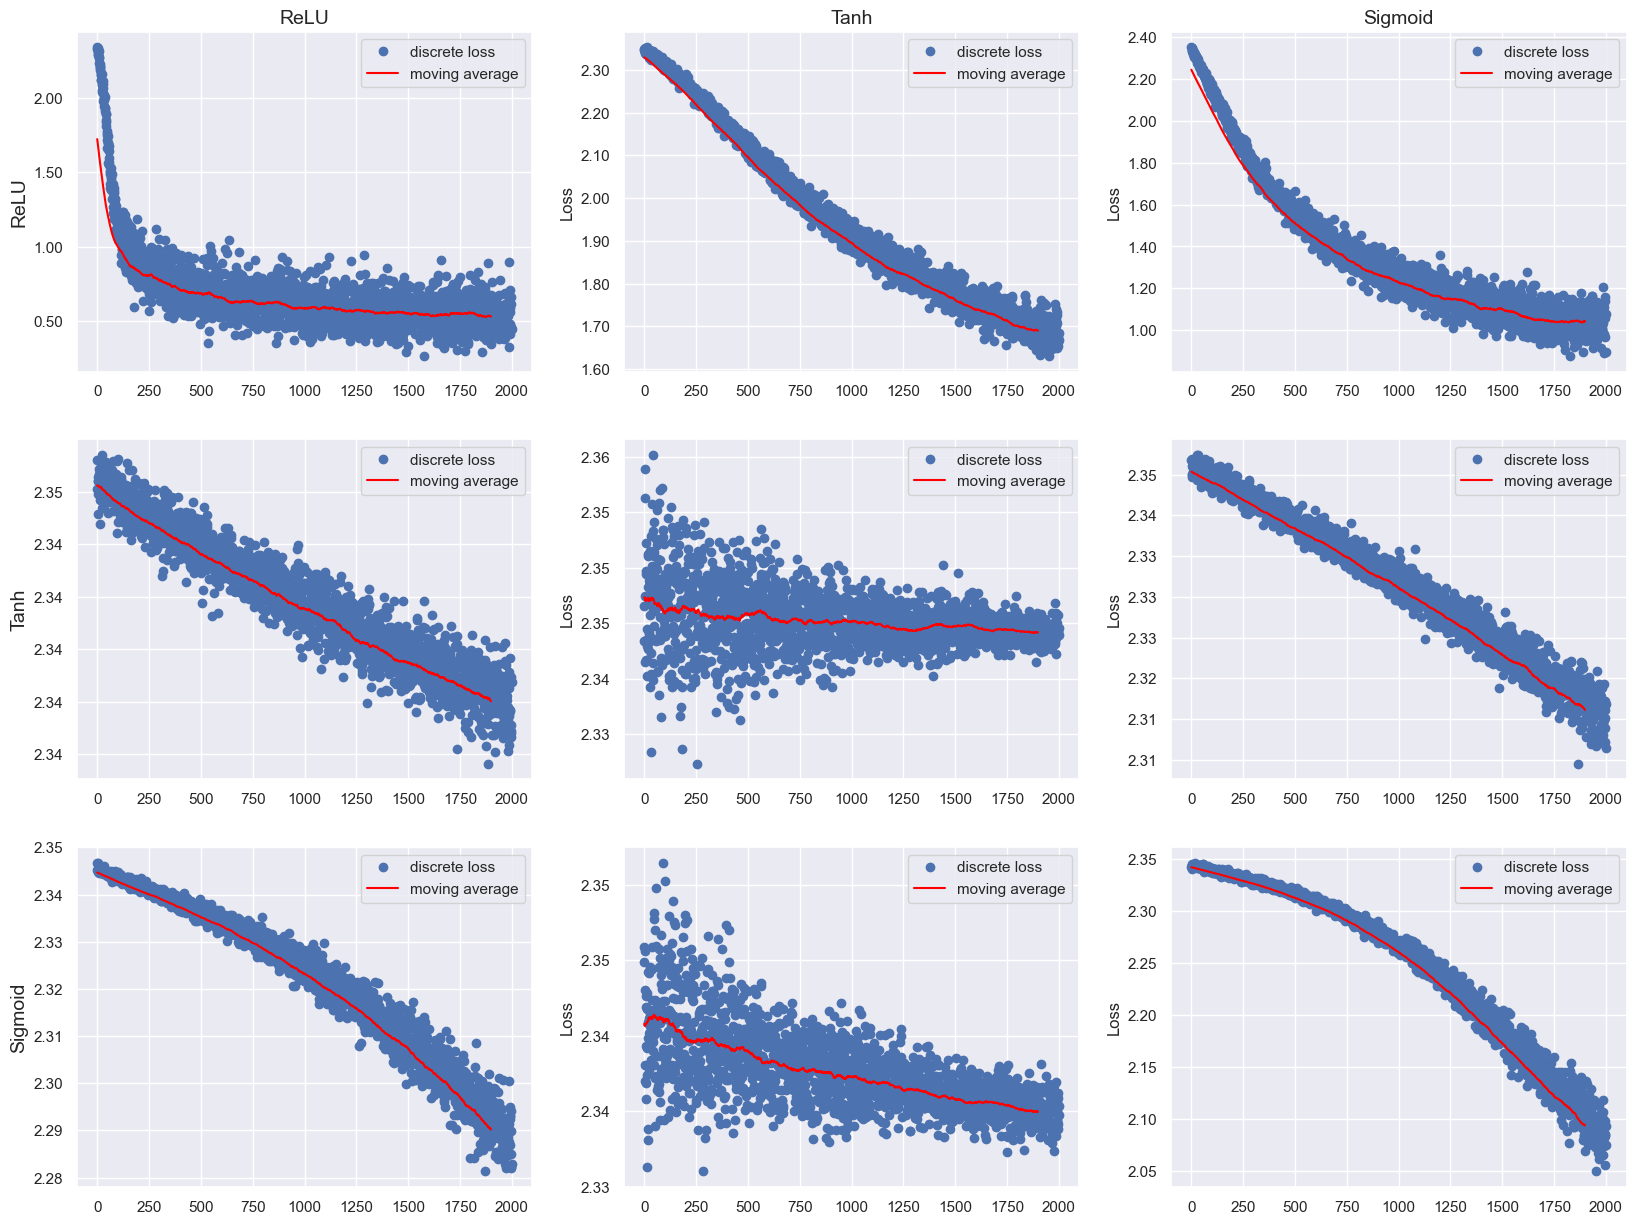
\includegraphics[scale=0.21]{images/activation_loss.png}
    \caption{Loss on different combinations of activation functions}
    \label{fig:activation-loss}
\end{figure}

\begin{figure}[htbp]
    \centering
    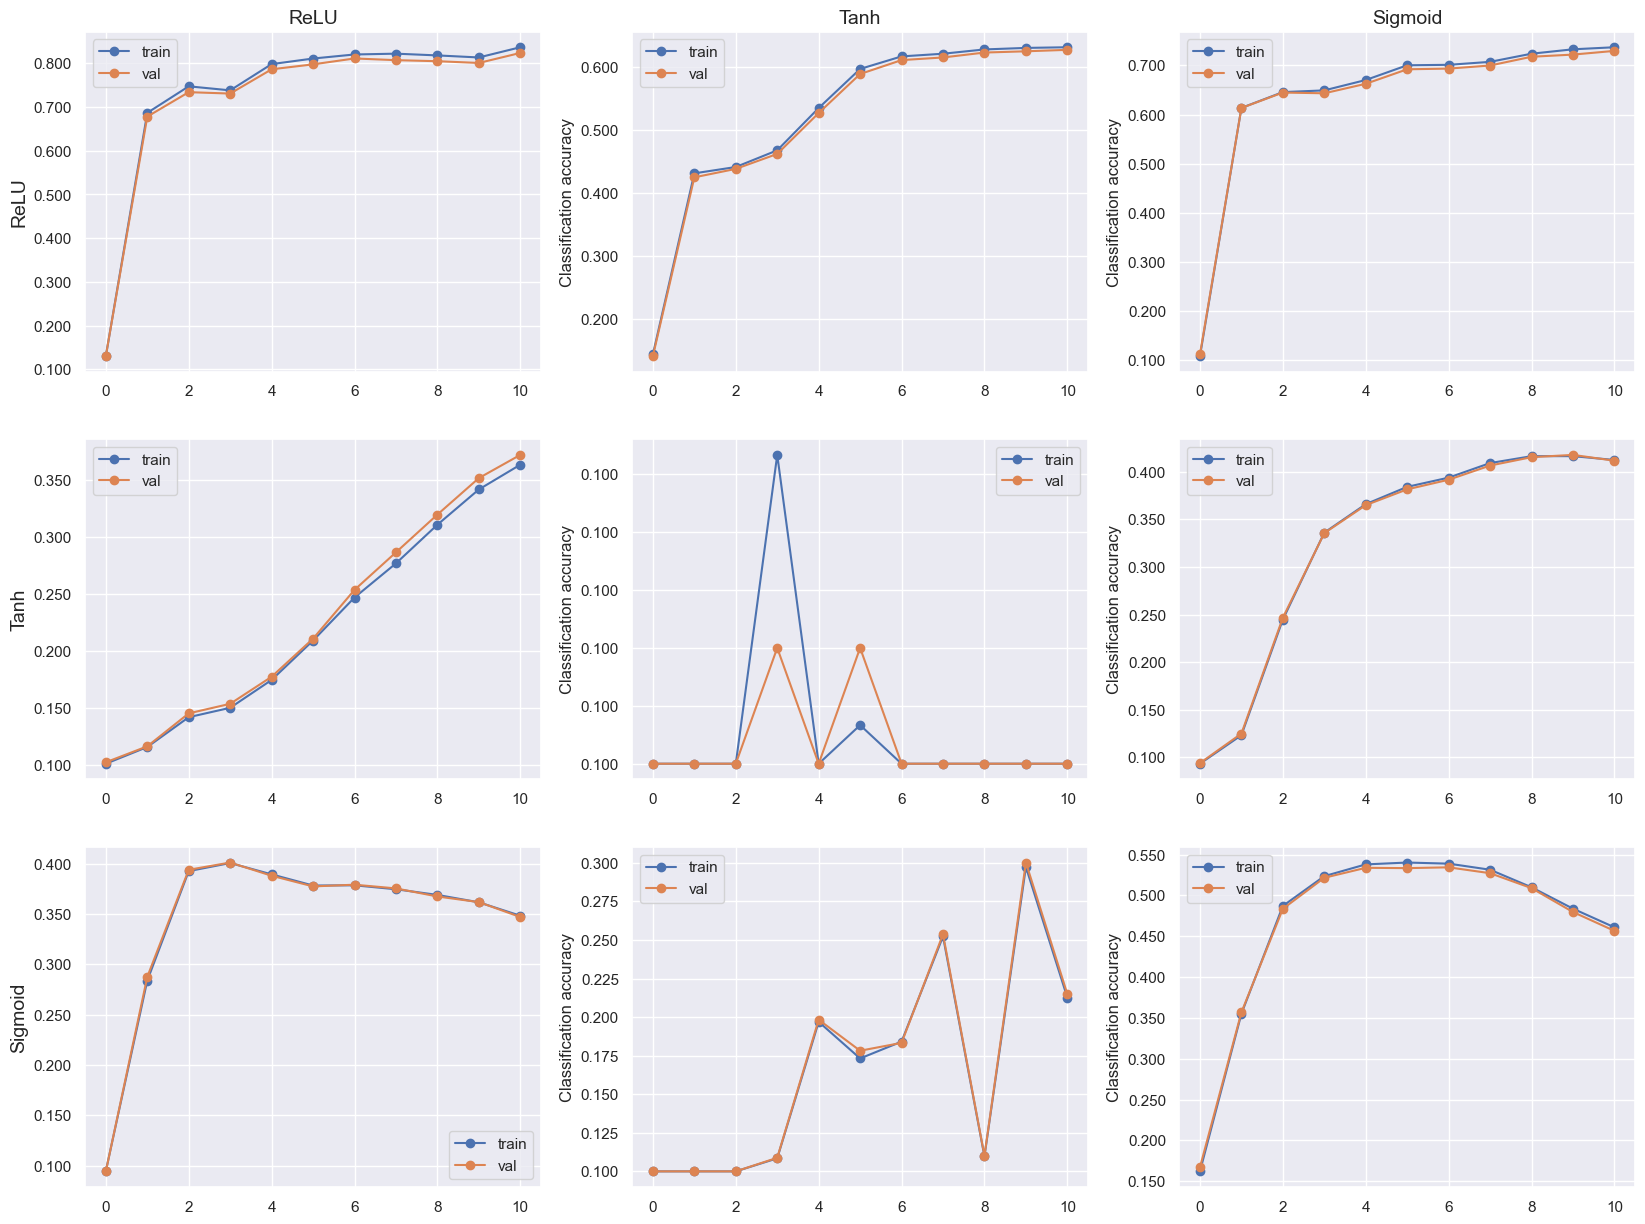
\includegraphics[scale=0.21]{images/activation_acc.png}
    \caption{Accuracy on different combinations of activation functions}
    \label{fig:activation-acc}
\end{figure}

Based on the results, we observe that the top three performing combinations are ['ReLU', 'ReLU'], followed by ['ReLU', 'Sigmoid'], and then ['ReLU', 'Tanh']. Notably, for combinations other than these top three, their loss remains consistently above 2 even after 2000 iterations. The superiority of \texttt{ReLU} over other activation functions is evident, likely attributed to mitigating the gradient vanishing problem present in both \texttt{Tanh} and \texttt{Sigmoid} functions.

Furthermore, it's noteworthy that when \texttt{ReLU} is exclusively applied in the second layer, performance degradation occurs. This observation suggests neural network saturation after the first activation layer if it's not implemented with \texttt{ReLU}. Consequently, we will proceed with the combination ['ReLU', 'ReLU'] in the subsequent sections.


\subsubsection{Tune Hyperparameters}

We will now employ a grid search method to fine-tune the parameters \texttt{hidden\_dims}, \texttt{learning\_rate}, and \texttt{reg}. Given a training dataset size of 60,000 with 10 labels, and to ensure generality and computational feasibility, we'll explore combinations of hidden dimensions such as 128, 64, and 48. For the remaining parameters, we'll adopt empirically optimal values. The results of the grid search are presented in the Table \ref{tab:grid-search-results} in Appendix \ref{subsec:grid-table}.

Upon examining the table, we observe that \texttt{hidden\_dims} and \texttt{reg} have slightly less impact on the loss compared to \texttt{learning\_rate}. The optimal learning rate may fall around $1e^{-2}$ since their validation accuracy are the highest on average.

To further fine-tune these parameters, we'll utilize a random search. For simplicity of visualization, we'll set the hidden dimensions as $[128, 64]$, randomly sample regularization values from $[1e^{-2.5}, 1e^{-2}]$, and learning rates from $[1e^{-3}, 1e^{-1.5}]$. The optimal parameters found in the former grid search are also added into the searching range of configuration. The precise search results are listed in the Table \ref{tab:random-search-results} in Appendix \ref{subsec:random-table} and visualized in the Figure \ref{fig:random-search}.

\begin{figure}[htbp]
    \centering
    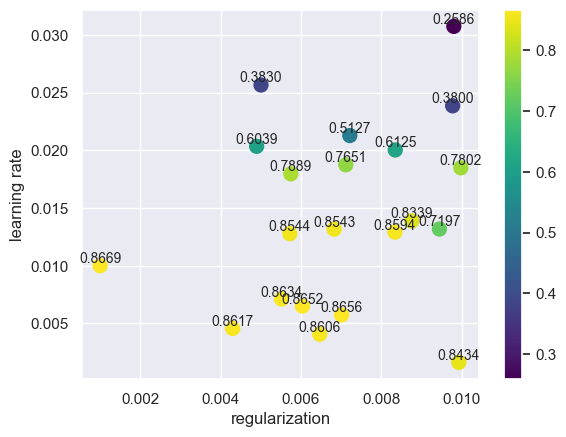
\includegraphics[scale=0.6]{images/random_search_scatter.png}
    \caption{Scatter plot of random search results}
    \label{fig:random-search}
\end{figure}

Combining the results from both the table and figure, it's evident that the validation accuracy increases as the learning rate increases from $1e^{-3}$ to approximately $1e^{-2}$, but decreases rapidly beyond this point. Hence, it's inferred that the optimal learning rate should be chosen around $1e^{-2}$.

To further substantiate the selection of the learning rate, we will fix the \texttt{reg} parameter at its optimal value and plot the loss history of neural networks with different manually selected learning rates. This comparison is depicted in Figure \ref{fig:lr-loss}. It is observable that a lower learning rate (0.0001) may result in a slower decay rate of the loss. Conversely, a high learning rate (0.03) could lead to escaping the saddle point of the loss function and increasing the loss as training progresses. Additionally, there are cases where a high learning rate may cause the loss to decrease too rapidly initially but plateau after several hundred iterations, maintaining a high loss in the end. Unfortunately, this phenomenon did not occur in our training process, which could be attributed to the dataset specifications and the choice of evaluation metrics beforehand.

In the end, the optimal parameters found after the two-phase search are \texttt{hidden\_dims} = [128, 64], \texttt{reg} = 0.001, and \texttt{learning\_rate} = 0.01.


\subsubsection{Applying Different Update Rules}

After obtaining the best parameters from the aforementioned procedures, we proceed to apply four different update rules, each with 2000 iterations. The loss history for each update rule is illustrated in Figure \ref{fig:update-rule}.

Clearly, the update rules, excluding SGD, demonstrate substantial enhancements, resulting in a hastened decay of the loss function.

\begin{figure}[htbp]
    \centering
    \begin{minipage}{0.45\textwidth}
        \centering
        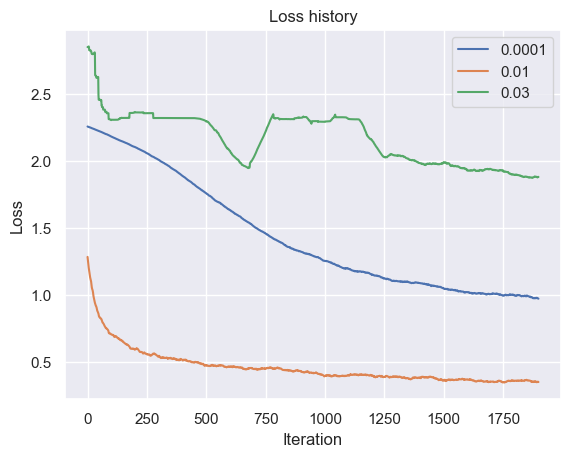
\includegraphics[width=0.9\textwidth]{images/learning_rate_loss.png}
        \caption{Loss history for different learning rates}
        \label{fig:lr-loss}
    \end{minipage}\hfill
    \begin{minipage}{0.45\textwidth}
        \centering
        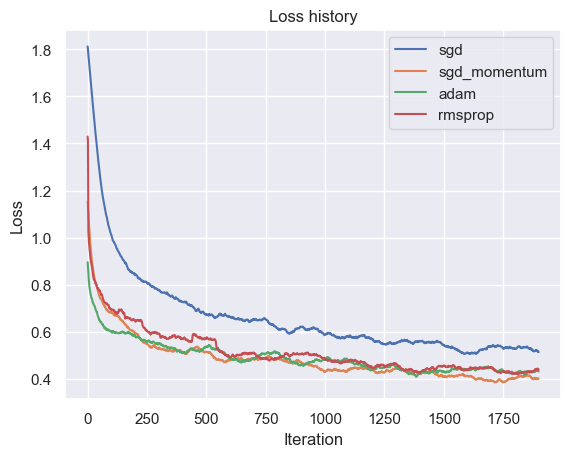
\includegraphics[width=0.9\textwidth]{images/update_rule_loss.png}
        \caption{Loss history of different update rules}
        \label{fig:update-rule}
    \end{minipage}
\end{figure}

\subsection{Training on Full Dataset}

Now that we have obtained the optimal hyperparameters, let's train our model on the full training dataset using these parameters. We'll run the training for 30,000 iterations, with other parameters set to their default values as specified in the comments for the \texttt{Solver} and \texttt{FullConnectNet} classes. Besides, the loss history and accuracy history during the training process are visualized in the accompanying Figure \ref{fig:full-train}. The training accuracy of the model reaches $94.8\%$ upon completion of the training process.

\begin{figure}[htbp]
    \centering
    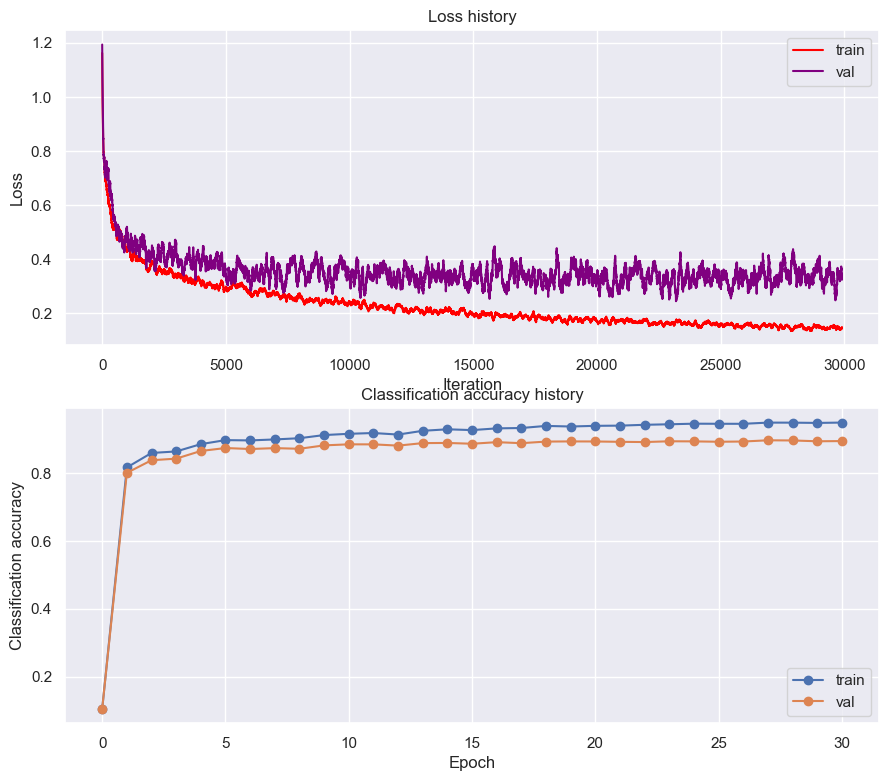
\includegraphics[scale=0.35]{images/full_train.png}
    \caption{Training on the Full Dataset}
    \label{fig:full-train}
\end{figure}

Once the training is completed, we save the trained model as a \texttt{.npz} file in the path \texttt{./model/fcnn.npz}.


\section{Load \& Test}

Having successfully trained the three-layer neural network and saved the weight parameters, we now proceed to load the trained model and evaluate its performance on the testing dataset. The accuracy table is presented in Table \ref{tab:accuracy-table} and the confusion matrix is visualized in Figure \ref{fig:confusion-matrix}.

\begin{table}[htbp]
\centering
\begin{tabular}{|c|c|c|c|}
    \hline
                &   Accuracy(Recall) &   Precision &   F1-score \\ \hline
    T-shirt/top &             0.85   &  0.843254   &   0.846614 \\ \hline
    Trouser     &             0.974  &  0.986829   &   0.980372 \\ \hline
    Pullover    &             0.823  &  0.809243   &   0.816063 \\ \hline
    Dress       &             0.898  &  0.887352   &   0.892644 \\ \hline
    Coat        &             0.819  &  0.81982    &   0.81941  \\ \hline
    Sandal      &             \textcolor{red}{0.976}  &  0.973081   &   0.974538 \\ \hline
    Shirt       &             \textcolor{blue}{0.726}  &  0.751553   &   0.738555 \\ \hline
    Sneaker     &             0.956  &  0.955045   &   0.955522 \\ \hline
    Bag         &             \textcolor{red}{0.976}  &  0.975025   &   0.975512 \\ \hline
    Ankle boot  &             0.966  &  0.960239   &   0.963111 \\ \hline
    \textcolor{orange}{Total}       &  \textcolor{orange}{0.8964}  &  \textcolor{orange}{0.896144}   &   \textcolor{orange}{0.896234} \\ \hline
\end{tabular}
\caption{Accuracy table}
\label{tab:accuracy-table}
\end{table}

\begin{figure}[htbp]
\centering
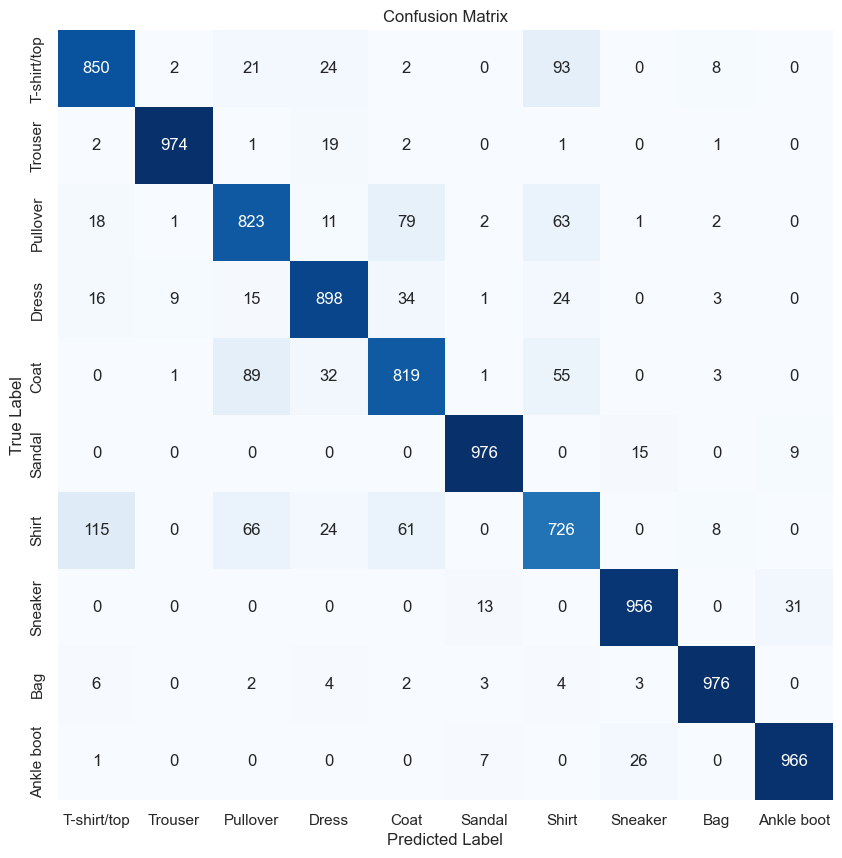
\includegraphics[scale=0.38]{images/confusion_matrix.png}
\caption{Confusion matrix}
\label{fig:confusion-matrix}
\end{figure}

The model achieves an accuracy of $89.64\%$ on the testing dataset. It performs exceptionally well on the labels "Sandal" and "Bag," with accuracies exceeding $97.5\%$. However, it struggles with the "Shirt" category, achieving an accuracy below $73\%$.

Examining the confusion matrix reveals notable misclassifications between "T-shirt/top" and "Shirt," as well as between "Pullover" and "Coat." These errors likely stem from the similarities in their shapes. Conversely, "Sandal" and "Bag" exhibit unique shapes, contributing to their high accuracy. This demonstrates that our neural network has indeed gleaned insightful knowledge about the dataset.

Next, we select 10 samples from each of the 10 labels and visualize them after passing through the first and second layers. This will provide us with some intuition about the trained neural network. The visualizations are depicted in Figures \ref{fig:original-image}, \ref{fig:first-layer}, and \ref{fig:second-layer}.

\begin{figure}[htbp]
\centering
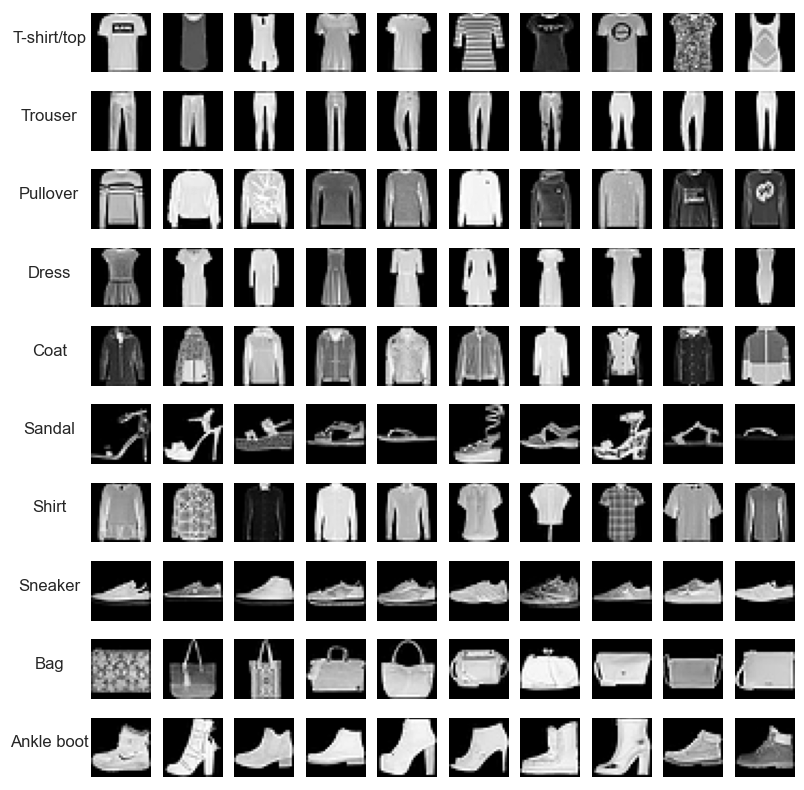
\includegraphics[scale=0.43]{images/original_image.png}
\caption{Original images}
\label{fig:original-image}
\end{figure}

\begin{figure}[htbp]
\centering
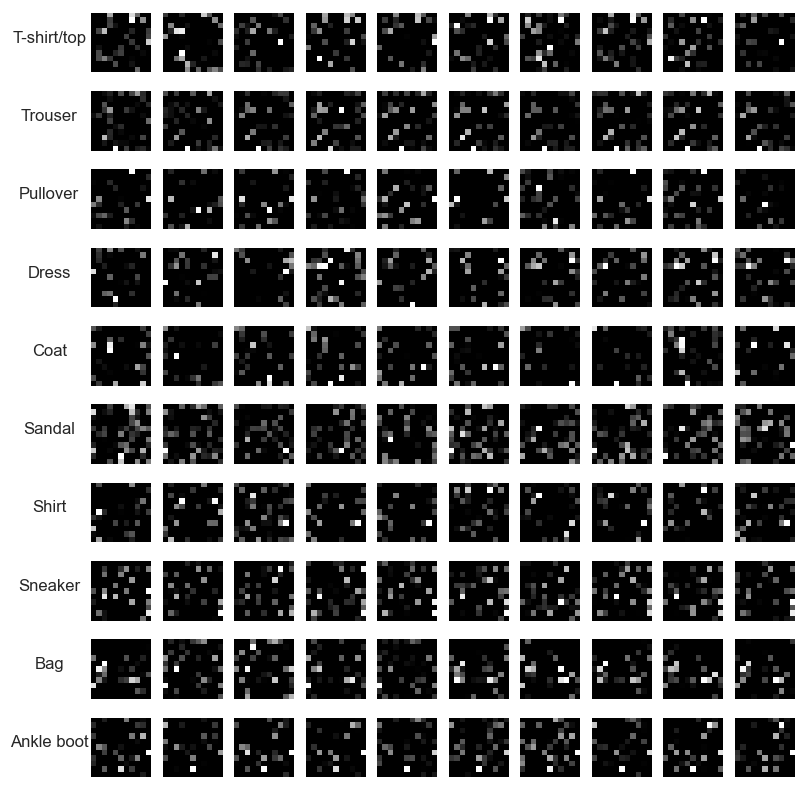
\includegraphics[scale=0.43]{images/first_layer.png}
\caption{Images after the first layer}
\label{fig:first-layer}
\end{figure}

\begin{figure}[htbp]
\centering
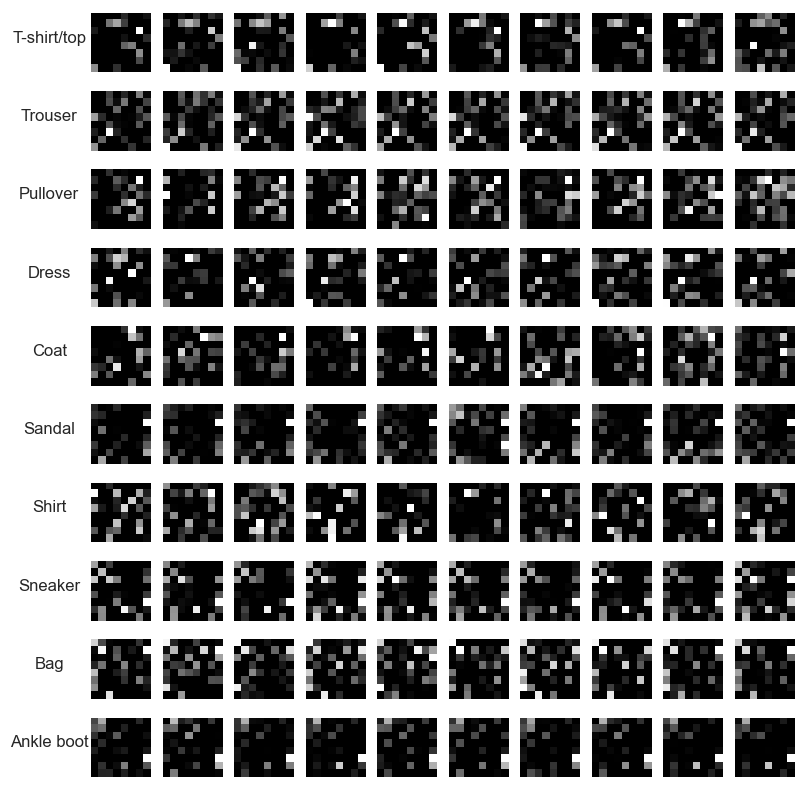
\includegraphics[scale=0.43]{images/second_layer.png}
\caption{Images after the second layer}
\label{fig:second-layer}
\end{figure}

Upon inspection, it's evident that the images after the first layer for each class lack significant similarity. This may be attributed to the neural network's insufficient learning of dataset features within a single layer. However, in the images after the second layer, distinct patterns for each class become apparent. Notably, the Sandal and Bag classes exhibit the most similarity among the selected 10 images, while the patterns for the Shirt class are less consistent, consistent with the observations in the accuracy table.

Lastly, the weights and biases of the trained neural network are depicted in Figure \ref{fig:weight-biases}. We observe that the absolute values of $\vec{W}_1$ and $\vec{W}_2$ are slightly lower than those of $\vec{W}_3$, potentially due to the combined effect of the $l_2$ penalty imposed on the weight matrices and gradient flow. Additionally, a discernible pattern emerges in each row or column of $\vec{W}_1$, characterized by alternating positive and negative values. This behavior suggests that the weight matrix may be capturing information related to edge detection in the image data. However, for $\vec{W}_2$ and $\vec{W}_3$, the patterns appear random and lack a clear explanation.

\begin{figure}[]
\centering
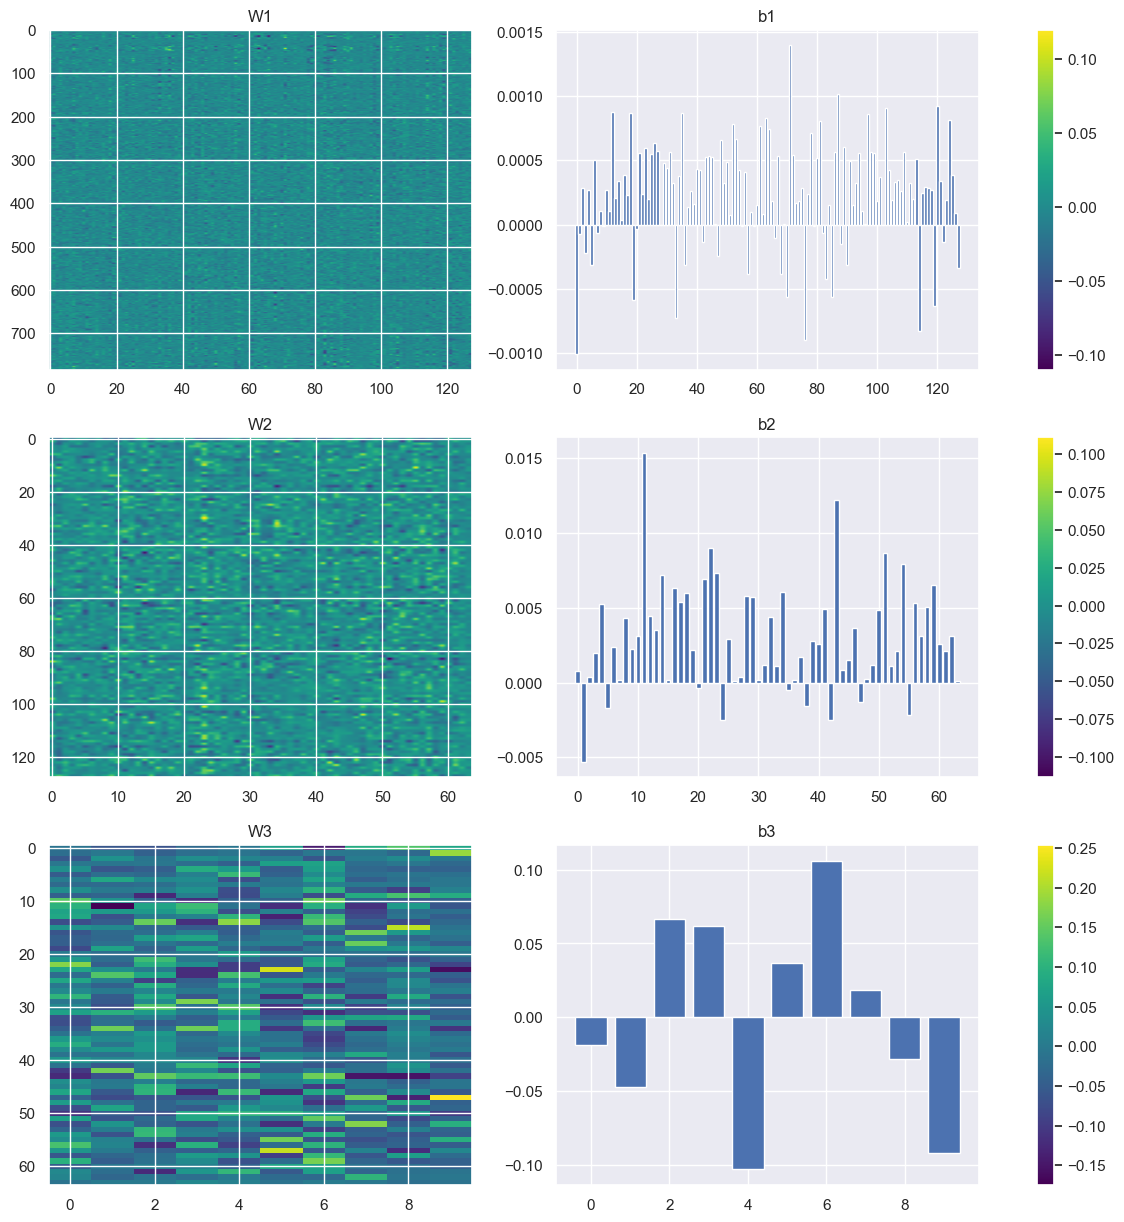
\includegraphics[scale=0.3]{images/weight_biases.png}
\caption{Weights and biases of the network}
\label{fig:weight-biases}
\end{figure}

\section{Discussion}

While our neural network has achieved relative good accuracy in classifying images from the Fashion-MNIST dataset, there are several areas where further refinement and exploration could potentially lead to even better performance and model robustness.

\subsection{Weight Initialization}

In this project, we briefly touched upon weight initialization in the neural network. In practice, various initialization methods like Xavier initialization and Kaiming initialization can significantly impact network performance. Exploring these methods could lead to improved results.

\subsection{Hyperparameter Tuning}

Although we provided hyperparameters such as \texttt{lr\_decay}, \texttt{batch\_size}, and \texttt{epochs}, we opted for their default values. However, fine-tuning these hyperparameters could potentially enhance the neural network's performance. Further investigation into optimal hyperparameter settings may yield better results.

\renewcommand{\thesubsection}{\Alph{subsection}} 
\newpage

\section{Appendix}

\subsection{Grid Search Results} \label{subsec:grid-table}

\begin{table}[h]
    \centering
    \begin{tabular}{|c|c|c|c|}
        \hline
        \texttt{hidden\_dims} & \texttt{reg} & \texttt{learning\_rate} & Val acc\\ \hline
        [128, 64] & 0.001 & 0.0001 & 0.6629 \\ \hline
        [128, 64] & 0.001 & 0.001  & 0.8312 \\ \hline
        [128, 64] & 0.001 & 0.01   & \textcolor{red}{0.8665} \\ \hline
        [128, 64] & 0.01  & 0.0001 & 0.6599 \\ \hline
        [128, 64] & 0.01  & 0.001  & 0.8279 \\ \hline
        [128, 64] & 0.01  & 0.01   & 0.8598 \\ \hline
        [128, 64] & 0.1   & 0.0001 & 0.6587 \\ \hline
        [128, 64] & 0.1   & 0.001  & 0.8222 \\ \hline
        [128, 64] & 0.1   & 0.01   & 0.8429 \\ \hline
        [128, 48] & 0.001 & 0.0001 & 0.6456 \\ \hline
        [128, 48] & 0.001 & 0.001  & 0.8298 \\ \hline
        [128, 48] & 0.001 & 0.01   & \textcolor{red}{0.8646} \\ \hline
        [128, 48] & 0.01  & 0.0001 & 0.6463 \\ \hline
        [128, 48] & 0.01  & 0.001  & 0.8286 \\ \hline
        [128, 48] & 0.01  & 0.01   & \textcolor{red}{0.8653} \\ \hline
        [128, 48] & 0.1   & 0.0001 & 0.6508 \\ \hline
        [128, 48] & 0.1   & 0.001  & 0.8240 \\ \hline
        [128, 48] & 0.1   & 0.01   & 0.8416 \\ \hline
        [64, 48] & 0.001 & 0.0001 & 0.6183 \\ \hline
        [64, 48] & 0.001 & 0.001  & 0.8172 \\ \hline
        [64, 48] & 0.001 & 0.01   & \textcolor{red}{0.8633} \\ \hline
        [64, 48] & 0.01  & 0.0001 & 0.6176 \\ \hline
        [64, 48] & 0.01  & 0.001  & 0.8186 \\ \hline
        [64, 48] & 0.01  & 0.01   & 0.8593 \\ \hline
        [64, 48] & 0.1   & 0.0001 & 0.6100 \\ \hline
        [64, 48] & 0.1   & 0.001  & 0.8100 \\ \hline
        [64, 48] & 0.1   & 0.01   & 0.8410 \\ \hline
    \end{tabular}
    \caption{Grid search results}
    \label{tab:grid-search-results}
\end{table}

\newpage
\subsection{Random Search Results} \label{subsec:random-table}
\begin{table}[h]
    \centering
    \begin{tabular}{|c|c|c|}
        \hline
        \texttt{reg} & \texttt{learning\_rate} & Val acc\\ \hline
        0.0083 & 0.02 & 0.6124 \\ \hline
        0.005 & 0.0257  & \textcolor{blue}{0.3829} \\ \hline
        0.0088 & 0.0139   & 0.8339 \\ \hline
        0.0057  & 0.018 & 0.7889 \\ \hline
        0.0072  & 0.0213  & 0.5127 \\ \hline
        0.0083  & 0.0129   & 0.8594 \\ \hline
        0.0065   & 0.0041 & 0.8606 \\ \hline
        0.007   & 0.0057  & 0.8655 \\ \hline
        0.0057   & 0.0128   & 0.8544 \\ \hline
        0.001 & 0.0185 & 0.7801 \\ \hline
        0.0043 & 0.0046  & 0.8617 \\ \hline
        0.0049 & 0.0203   & 0.6039 \\ \hline
        0.0094  & 0.0132 & 0.7196 \\ \hline
        0.006  & 0.0065  & 0.8651 \\ \hline
        0.0071  & 0.0187   & 0.7650 \\ \hline
        0.0055   & 0.0071 & 0.8634 \\ \hline
        0.0098   & 0.0307  & \textcolor{blue}{0.2586} \\ \hline
        0.0068   & 0.0132   & 0.8542 \\ \hline
        0.0098 & 0.0239 & \textcolor{blue}{0.3799} \\ \hline
        0.0099 & 0.0016  & 0.8464 \\ \hline
        0.001 & 0.01   & \textcolor{red}{0.8668} \\ \hline
    \end{tabular}
    \caption{Random search results}
    \label{tab:random-search-results}
\end{table}
					
%----------------------------------------------------------

\addcontentsline{toc}{section}{References}
\printbibliography

%----------------------------------------------------------


\end{document}